\documentclass{article}
\title{CSC352 HW9}
\author{Alex Zhang}
\date{April 2023}
\textwidth=16.00cm 
\textheight=22.00cm 
\topmargin=0.00cm
\oddsidemargin=0.00cm 
\evensidemargin=0.00cm 
\headheight=0cm 
\headsep=0.5cm
\textheight=610pt
\usepackage{graphicx}

\graphicspath{ {./images/} }

\usepackage{latexsym,array,delarray,amsthm,amssymb,epsfig,amsmath,listings}

\lstset{
  basicstyle=\ttfamily,
  mathescape
}

\newcommand{\bmat}[1]{\begin{bmatrix} #1 \end{bmatrix}}
\newcommand{\mat}[1]{\mathbf{#1}}

\let\ds\displaystyle

\begin{document}
\maketitle
\section*{Question 1}
Based on obvervation, I find out matrix $\mat{A}$ is a quasi-upper triangular matrix.
\begin{center}
    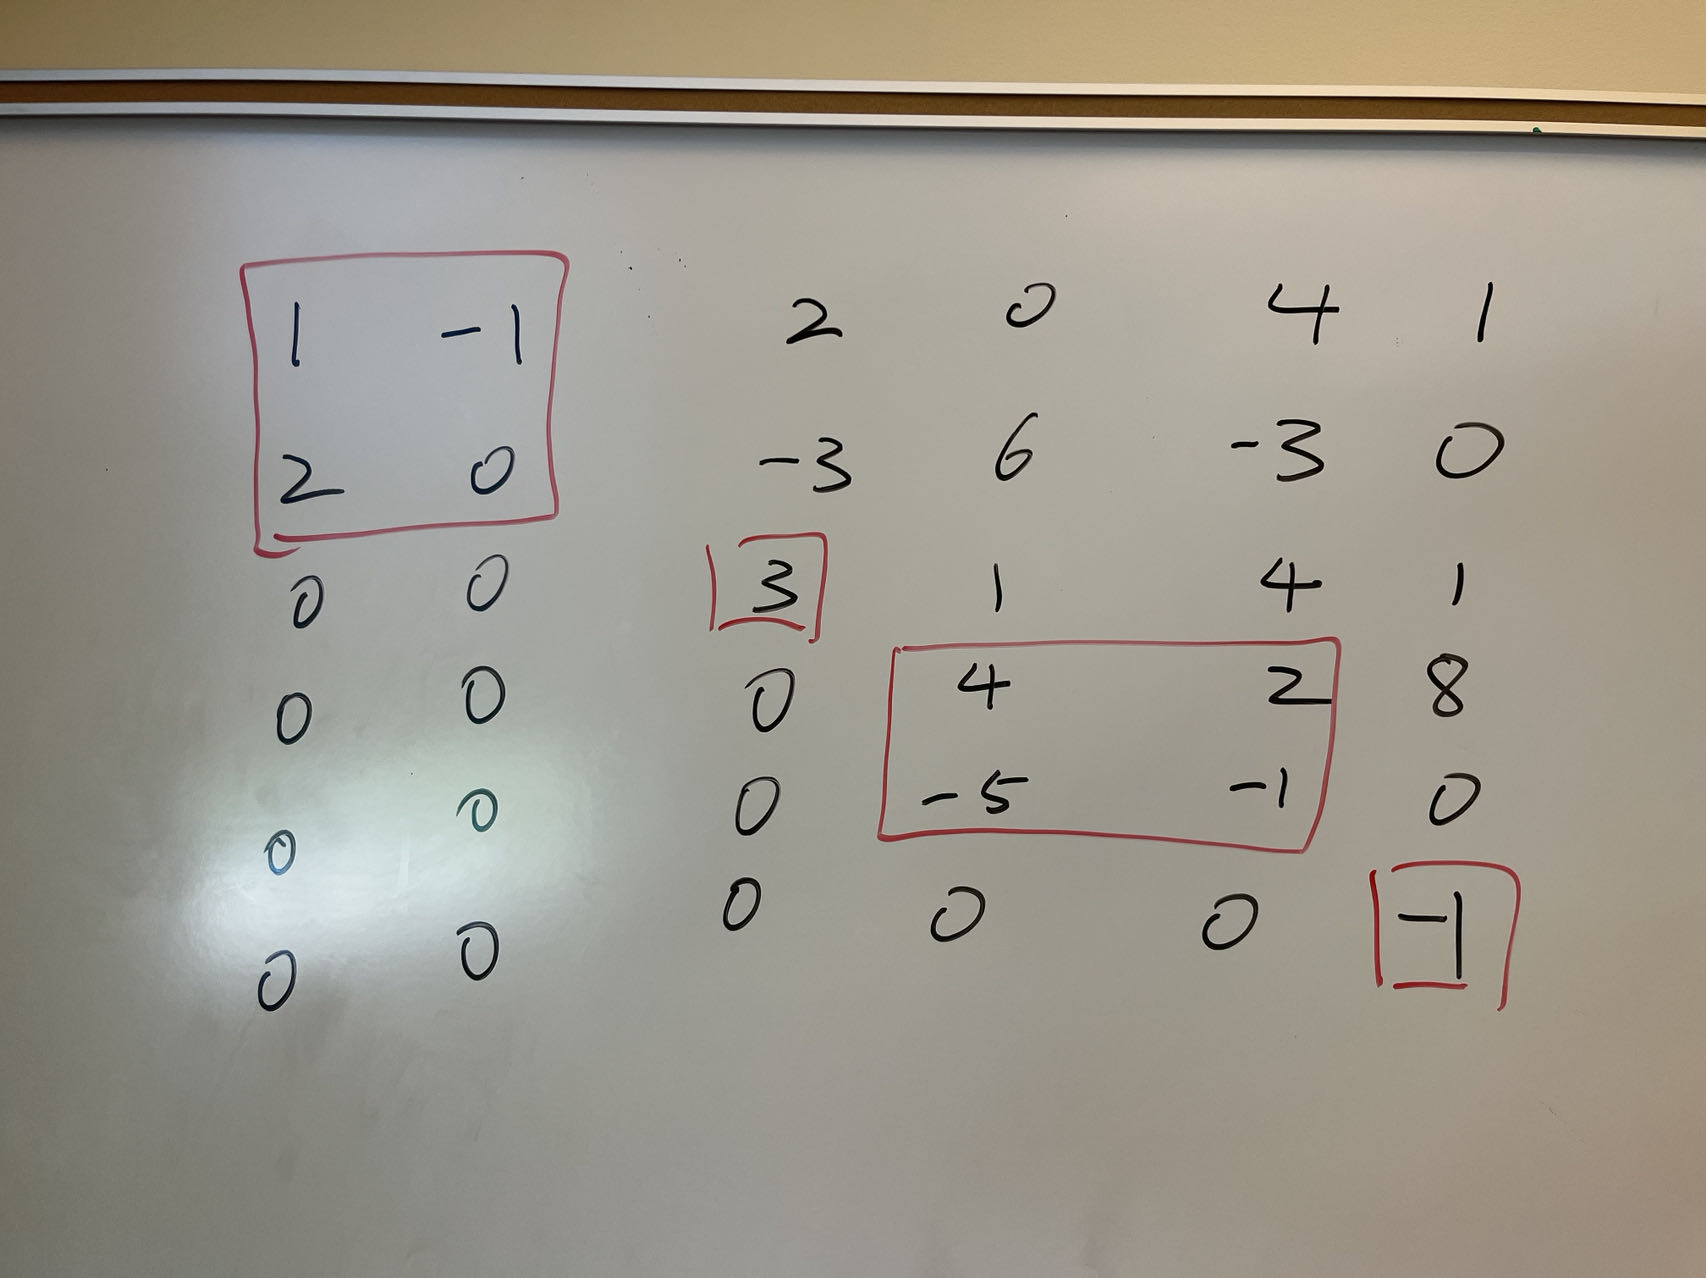
\includegraphics[scale = 0.2]{quasi.jpg}
\end{center}
which I can do real schur decomposition on $\mat{A}$ which $\mat{A} = \mat{I}\mat{A}\mat{I}^\top$.
$\mat{I}$ is identity matrix with same dimension of $\mat{A}$, and they are orthorgonal matrix. Therefore we can first get 
two eigenvalues $3$ and $-1$. Then I will calculate the eigenvalues for rest two 2 by 2 matrices.


\section*{Question 2}
The pseudocode for Golub Kahan bidiagonalization will is below:

\begin{verbatim}
    function B = GK_bidiagonalization(A)
        [m,n] = size(A)
        for j = 1:n
            x = A(j:m, j)
            u = x + norm(x) * e1
            u = u / norm(u)
            A(j:m,j:n) = A(j:m,j:n) - 2 * u * (u' * A(j:m,j:n))
            if j < n-1
                x = A(j, j+1:m)
                v = x + norm(x) * e1
                v = v / norm(v)
                A(j:m, j+1:n) = A(j:m, j+1:n) - 2 * (A(j:m, j+1:n) * v) * v'
            end if    
        B = A
    end function
\end{verbatim}

\section*{Question 4}
\subsection*{(a)}
After doing SVD on $\mat{A}$, the first singular value is $156.4358$ and the second one is $8.7658$. I think 
becuase the largest singular value is way bigger than the rest. There will be
one principal component that relates to the first singular value.
\subsection*{(b)}

The rank-one approximation for matrix $\mat{A}$ will be, 
$$A_1 = \bmat{ 46.7021 &  15.8762\\
94.0315 &  31.9657 \\
52.0806  & 17.7046\\
43.3857  & 14.7488\\
68.2871  & 23.2139\\
40.6964  & 13.8346}$$
The relative error is $0.056$. Based on the result, I think this is kind of a good
approximation.

\subsection*{(c)}
I created two bar charts and find out that for height column, the approximated 
data is closer to true data with greatest difference by $1.7$. For weight column,
the approximated data is not so accurate compared to height's data. It has maximum difference 
by $4.75$.









$$z = v' * A(:,J)$$
$$z = $$

\end{document}